\chapter{Understanding the Limits of Direct Reinforcement Learning}

From the previous Chapter (cite) we know that to directly learn decision trees for an MDP, one can learn a deterministic partially observable policy for an IBMDP (cite).
Such problems are classical instances of partially observable Markov decision processes (POMDPs)~\cite{POMDP}. This connexion with POMDPs brings novel insights to direct reinforcement learning of decision tree policies. 
In this chapter, all the decision processes presented have a finite number of vector-valued states and observations. Hence we will use bold fonts for states and observations but can still use summations rather than integrals when required.

\subsection{Partially Observable IBMDPs}
A POMDP is an MDP where the current state is hidden; only some information about the current state is observable.

\begin{definition}[Partially Observable Markov Decision Processes]
A partially observable Markov decision process is a tuple $\langle X, A, O, T, T_0, \Omega, R\rangle$ where:
\begin{itemize}
    \item $X$ is the state space (like in the definition of MDPs (cite)).
    \item $A$ is a finite set of actions (like in the definition of MDPs(cite)).
    \item $O$ is a set of observations.
    \item $T: X \times A \rightarrow \Delta X$ is the transition kernal, where $T(boldsymbol{x}_t, a, \boldsymbol{x}_{t+1}) = P(\boldsymbol{x}_t|\boldsymbol{x}_{t+1}, a)$ is the probability of transitioning to state $\boldsymbol{x}_{t}$ when taking action $a$ in state $\boldsymbol{x}$
    \item $T_0$: is the intial distribution over states. 
    \item $\Omega: X \rightarrow \Delta O$ is the observation kernel, where $\Omega(\boldsymbol{o}, a, \boldsymbol{x}) = P(\boldsymbol{o}|\boldsymbol{x}, a)$ is the probability of observing $\boldsymbol{o}$ in state $\boldsymbol{x}$
    \item $R: X \times A \rightarrow \mathbb{R}$ is the reward function, where $R(\boldsymbol{x}, a)$ is the immediate reward for taking action $a$ in state $\boldsymbol{x}$
\end{itemize}
Note that $\langle X, A, R, T, T_0 \rangle$ defines an MDP (cite).
\end{definition}

Let us define explicitely a partially observable iterative bounding Markove decision process (POIBMDP). It is essentially an IBMDP extended with an observation space and an observation kernel:
\begin{definition}[Partially Observable Iterative Bounding Markov Decision Processes] a partially observable iterative bounding Markov decision process is an IBMDP (cite) is a tuple $\mathcal{M}_{POIB}$
    \begin{align*}
        \langle \overbrace{S\times \underbrace{O}_{\text{Observations}}}^{\text{fully observable states}}, \underbrace{A\cup A_{info}}_{Action space}, \overbrace{(R, \zeta)}^{Rewards}, \underbrace{(T_{info}, T, T_0)}_{Transitions}, \Omega \rangle
    \end{align*}
    Note that $\langle S\times O, A\cup A_{\info}, (R, \zeta),( T, T_0, T_{info})\rangle$ is an IBMDP (cite).
    The transition kernel $\Omega$ maps state features and observations to observations, $\Omega:S\times O \rightarrow O$, with $P(\boldsymbol{o}|(\boldsymbol{s}, \boldsymbol{o}))=1$ 
\end{definition}

One can see POIBMDPs as a particular instance of POMDPs where the observation kernel simply applies a mask over some features of the fully observable state.
This setting has other names in the litterature: Mixed Observability MDPs (cite), Block MDPs (cite) N-MDPs (cite).
POIBMDPs can also be seen as non-stationary MDPs in which there is one different transition kernel per base MDP state: these are called Hidden-Mode MDPs (cite). 

Following (cite) we can write the definition of the value of a deterministic partially observable policy $\pi:O\rightarrow A$ in observation $\boldsymbol{o}$.

\begin{definition}[Partially observable value function] In a POIBMDP, the expected cumulative discounted reward of a deterministic partially observable policy $\pi:O\rightarrow A\cup A_{info}$ starting from observation $o$ is $V^{\pi}(\boldsymbol{o})$:
    \begin{align*}
        V^{\pi}(\boldsymbol{o}) &= \underset{(s,\boldsymbol{o}')\in S\times O}{\sum}P^{\pi}((s, \boldsymbol{o}')|\boldsymbol{o})V^{\pi}((s, \boldsymbol{o}'))
    \end{align*}
with $P^{\pi}((s, \boldsymbol{o}')|\boldsymbol{o})$ the asymptotic occupancy distribution (see cite for definition) of the fully observable state $(s,\boldsymbol{o}')$ given the partial observation $o$ and $V^{\pi}((s, o'))$ the classical state-value function defined in (cite).
\end{definition}

The asymptotic occupancy distribution is the probability of a policy $\pi$ to be in $(s,\boldsymbol{o}')$ while observing $\boldsymbol{o}$ and having taken actions given by $\pi$.  
We can re-write the Direct interpretable RL objective (cite) in terms of POIBMDPs:

\begin{definition}[Revised Direct interpretable RL objective]
    Given an MDP $\mathcal{M}$ (cite) and an associated POIBMDP $\mathcal{M}_{POIB}$(cite), the direct interpretable RL objective is:
\begin{align}
    \pi^{\star} &= \underset{\pi}{\operatorname{argmax}}J(\pi) = \underset{\pi}{\operatorname{argmax}}V^{\pi}(\boldsymbol{o}_0)
\end{align}
With $\pi$ a determintic partially observable policy $\pi:O\rightarrow A\cup A_{info}$. There is no expectation over possible initial observation in the above objective function as there is only one initial observation in a POIBMDP: $o_0=(L_1, U_1, \dots, L_n, U_n)$ (cite).
\end{definition}

In this Chapter, we use (asymmetric) reinforcement learning to train decision tree policies for MDPs by seeking deterministic partially observable policies for POIBMDPs (cite), i.e. by solving (cite).  

\begin{figure}[h]
\centering
\begin{tikzpicture}
    \draw[fill=blue!40] (0, 0) rectangle (6, 4);
    \node at (3, 3.5) {POIBMDP $\mathcal{M}_{POIB}\langle\mathcal{M}_{IB}, \Omega\rangle$};
    \draw[fill=blue!30] (0, 0) rectangle (5.9, 3);
    \node at (3, 2.5) {IBMDP $\mathcal{M}_{IB} \langle \mathcal{M}, O, A_{info}, \zeta, T_{info}\rangle$};
    \draw[fill=blue!10] (0, 0) rectangle (5, 2);
    \node at (3, 1.5) {MDP $\mathcal{M} \langle S, A, R, T, T_0 \rangle$};
    
    \draw[fill=red!10] (10, 0) rectangle (14, 3);
    \node at (12, 2) {\textbf{Objective}};
    \node at (12, 1) {$\pi^{\star} = \underset{\pi}{\operatorname{argmax}} V^{\pi}(o_0)$};
    
    \draw[fill=red!10] (1, -5) rectangle (5, -2);
    \node at (3, -3) {\textbf{Decision Tree Policy}};
    \node at (3, -4) {$\pi_{\mathcal{T}}: S \rightarrow A$};
    
    \draw[fill=red!10] (9.5, -5) rectangle (14.5, -2);
    \node at (12, -3) {\textbf{Deterministic PO Policy}};
    \node at (12, -4) {$\pi: O \rightarrow A \cup A_{info}$};
    
    \draw[thick, ->] (6, 2) -- (10, 2) node[midway, above] {$\gamma$};
    \draw[thick, <-] (5, -3.5) -- (9.5, -3.5) node[midway, above] {Extract tree with Alg 6};
    \draw[thick, ->] (12, 0) -- (12, -2) node[midway, left] {Solve with e.g. RL};
    \draw[thick, <-] (3, 0.5) -- (3, -2) node[midway, left] {Can be interpreted};

    
    % % Final arrow from tree back to base MDP - adjusted position
    % \draw[thick, ->] (1.75, -2.5) -- (1.75, -0.5) node[midway, right] {Can deploy\\and interpret};
    
\end{tikzpicture}
\caption{A formal framework to learn decision tree policies for MDPs that directly optimize the RL objective (cite). This include learning a partially observable deterministic policy in a POIBMDP (cite).}
\label{fig:nested_decision_processes}
\end{figure}

We will attempt to \textit{learn} the optimal--w.r.t the RL objective (cite)--depth-1 tree policy from Figure (cite) for the $2\times 2$ grid world from Example (cite).
We formulate this as solving the (revised) direct interpretble RL objective (cite) where the base MDP is the grid world and the POIBMDP is obtained from the IBMDP of Example (cite).

We choose $\gamma$ and $\zeta$ in the POIBMDP such that the \textit{optimal} partially observable deterministic policy, i.e. the solution to (cite), corresponds exactly to the decision tree of depth 1 from Figure (cite)
This depth 1 tree is in turn optimal in the grid world MDP w.r.t to the base RL objective (cite).
Next we present some insights about the solution space of (cite).

\section{Constructing POIBMDPs which optimal solutions are the depth-1 tree}
\begin{figure}[htbp]
    \centering
    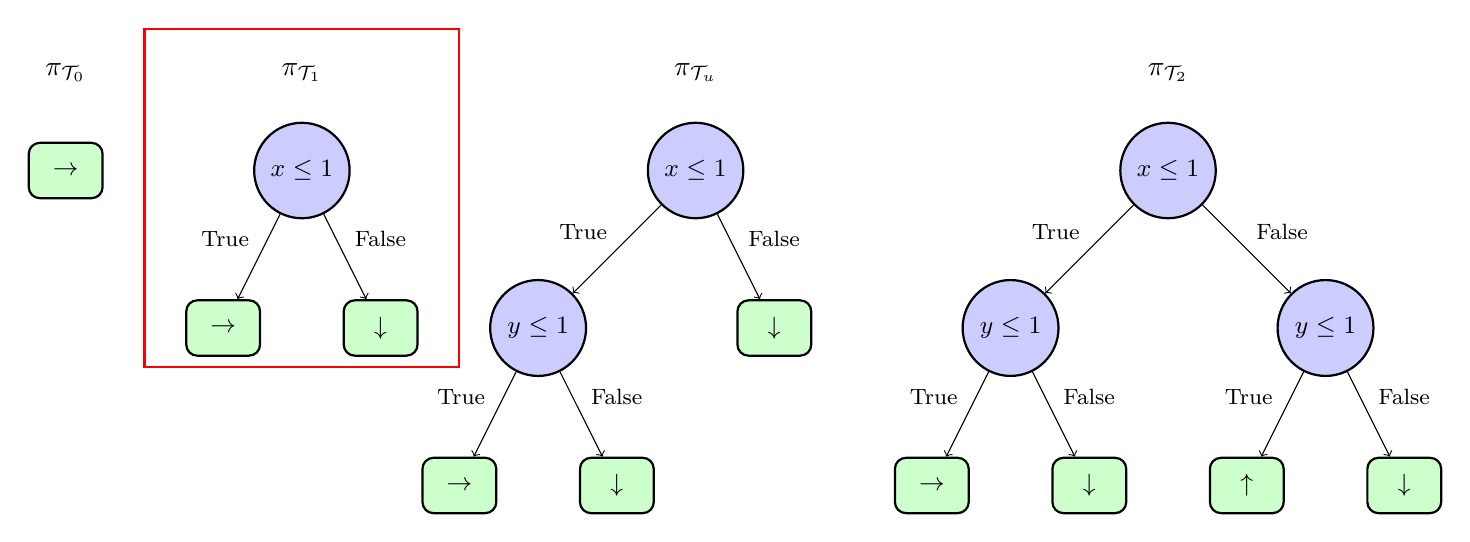
\begin{tikzpicture}[
        scale=1,
        decision/.style={circle, draw, thick, fill=blue!20, text width=2.5em, text centered, minimum height=2.5em, font=\small},
        leaf/.style={rectangle, draw, thick, fill=green!20, text width=2em, text centered, rounded corners, minimum height=2em, font=\small},
        edge_label/.style={font=\footnotesize, midway}
    ]
        
        \node[leaf] at (-3, 0) {$\rightarrow$};
        % Tree 4: if x <= 0.5 move right else move left
        \node[decision] (tree4_root) at (0,0) {$x \leq 1$};
        \node[leaf] (tree4_right) at (-1,-2) {$\rightarrow$};
        \node[leaf] (tree4_left) at (1,-2) {$\downarrow$};
        \draw[->] (tree4_root) -- (tree4_right) node[edge_label, above left] {True};
        \draw[->] (tree4_root) -- (tree4_left) node[edge_label, above right] {False};
        
        % Draw a square around the tree
        \draw[thick, red] (-2, 1.8) rectangle (2, -2.5);

        % Tree 7: if x <= 0.5 and y <= 0.5 move right else move down
        \node[decision] (tree7_root) at (5,0) {$x \leq 1$};
        \node[decision] (tree7_y) at (3,-2) {$y \leq 1$};
        \node[leaf] (tree7_right) at (2,-4) {$\rightarrow$};
        \node[leaf] (tree7_down) at (4,-4) {$\downarrow$};
        \node[leaf] (tree7_down2) at (6,-2) {$\downarrow$};
        \draw[->] (tree7_root) -- (tree7_y) node[edge_label, above left] {True};
        \draw[->] (tree7_root) -- (tree7_down2) node[edge_label, above right] {False};
        \draw[->] (tree7_y) -- (tree7_right) node[edge_label, above left] {True};
        \draw[->] (tree7_y) -- (tree7_down) node[edge_label, above right] {False};


        \node[decision] (tree7_root) at (11,0) {$x \leq 1$};
        \node[decision] (tree7_y) at (9,-2) {$y \leq 1$};
        \node[decision] (tree7_y2) at (13,-2) {$y \leq 1$};
        \node[leaf] (tree7_right) at (8,-4) {$\rightarrow$};
        \node[leaf] (tree7_down) at (10,-4) {$\downarrow$};
        \node[leaf] (tree7_right2) at (12,-4) {$\uparrow$};
        \node[leaf] (tree7_down2) at (14,-4) {$\downarrow$};
        \draw[->] (tree7_root) -- (tree7_y) node[edge_label, above left] {True};
        \draw[->] (tree7_root) -- (tree7_y2) node[edge_label, above right] {False};
        \draw[->] (tree7_y) -- (tree7_right) node[edge_label, above left] {True};
        \draw[->] (tree7_y) -- (tree7_down) node[edge_label, above right] {False};
        \draw[->] (tree7_y2) -- (tree7_right2) node[edge_label, above left] {True};
        \draw[->] (tree7_y2) -- (tree7_down2) node[edge_label, above right] {False};

        % Labels
        \node[above] at (-3,1) {$\pi_{\mathcal{T}_0}$};
        \node[above] at (0,1) {$\pi_{\mathcal{T}_1}$};
        \node[above] at (5,1) {$\pi_{\mathcal{T}_u}$};
        \node[above] at (11,1) {$\pi_{\mathcal{T}_2}$};


    \end{tikzpicture}
    \caption{For each decision tree structure, e.g., depth-1 or unbalanced depth-2, in the space of deterministic partially observable POIBMDP policies, we illustrate the decision tree which gets the highest base rewards.}
    \label{fig:optimal-policy-trees}
\end{figure}

Because we know all the base states, all the observations, all the actions, all the rewards and all the transitions of our POIBMDP, we can compute exactly the values of different partially observable deterministic policies given $\zeta$ the reward for IGAs and $\gamma$ the discount factor.

Each of those policies can be one of the following trees illustrated in Figure (cite): 
\begin{itemize}
    \item $\pi_{\mathcal{T}_0}$: a depth-0 tree equivalent to always taking the same base action 
    \item $\pi_{\mathcal{T}_1}$: a depth-1 tree equivalent alternating between an IGA and a base action 
    \item $\pi_{\mathcal{T}_u}$: an unbalanced depth-2 tree that sometimes takes two IGAs then a base action and sometimes a an IGA then a base action
    \item $\pi_{\mathcal{T}_2}$: a depth-2 tree that alternates between taking two IGAs and a base action
    \item an inifinite ``tree'' that only takes IGAs
\end{itemize}
Furthermore, because from (cite) we know that for POMDPs, stochastic policies can sometimes get better expected discounted rewards than deterministic policies, we also compute the value of the stochastic policy that alternates between two base actions: $\rightarrow$ and $\downarrow$.
Those two base actions always lead to the goal state in expectation.

We detail the calculations for the detpth-1 decision tree objective value (cite) and defer the calculations for the other policies to the Appendix (cite).

\begin{proposition}[Depth-1 decision tree objective value] The objective value of the best depth-1 decision tree from Figure (cite) is $V^{\pi_{\mathcal{T}_1}}(o_0) = \frac{4\zeta + \gamma + 2\gamma^3 + \gamma^5}{4(1-\gamma^2)}$.
\end{proposition}

\begin{proof} $\pi_{\mathcal{T}_1}$ has one root node that tests $x\leq1$ (respectively $y\leq1$) and two leaf nodes $\rightarrow$ and $\downarrow$. 
To compute $V^\pi_{\mathcal{T}_1}(o_0)$, we compute the values of $\pi_{\mathcal{T}_1}$ in each of the possible startin states $(s_0, o_0), (s_1, o_0), (s_2, o_0), (s_g, o_0)$ and compute the expectation over those. 
At inititalization, when the base state is $s_g = (1.5, 0.5)$, the depth-1 decision tree policy cycles between taking an information gathering action $x\leq1$ and moving down to get a positive reward for which it gets the returns:
\begin{align*}
    V^{\pi_{\mathcal{T}_1}} (s_g, o_0) &= \zeta + \gamma + \gamma^2 \zeta + \gamma^3 \dots \\
    &= \overset{\infty}{\underset{t=0}\sum} \gamma^{2t} \zeta + \overset{\infty}{\underset{t=0}\sum} \gamma^{2t+1} \\
    &= \frac{\zeta + \gamma}{1 - \gamma^2}
\end{align*}
At inititialization, in either of the base states $s_0=(0.5,0.5)$ and $s_2=(1.5, 1.5)$, the value of the depth-1 decision tree policy is the return when taking one information gathering action $x\leq1$, then moving right or down, then following the policy from the goal state $s_g$:
\begin{align*}
    V^{\pi_{\mathcal{T}_1}} (s_0, o_0) &= \zeta + \gamma 0 + \gamma^2 V^{\pi_{\mathcal{T}_1}} (s_g, o_0) \\
    &= \zeta + \gamma^2 V^{\pi_{\mathcal{T}_1}} (s_g, o_0) \\
    &= V^{\pi_{\mathcal{T}_1}} (s_2, o_0)
\end{align*}
Similarly, the value of the best depth-1 decision tree policy in state $s_1=(0.5,1.5)$ is the value of taking one information gathering action then moving right to $s_2$ then following the policy in $s_2$:
\begin{align*}
    V^{\pi_{\mathcal{T}_1}} (s_1, o_0) &= \zeta + \gamma 0 + \gamma^2 V^{\pi_{\mathcal{T}_1}} (s_2, o_0) \\
    &= \zeta + \gamma^2 V^{\pi_{\mathcal{T}_1}} (s_2, o_0) \\
    &= \zeta + \gamma^2 (\zeta + \gamma^2 V^{\pi_{\mathcal{T}_1}} (s_g, o_0)) \\
    &= \zeta + \gamma^2 \zeta + \gamma^4 V^{\pi_{\mathcal{T}_1}} (s_g, o_0)
\end{align*}
Since the probability of being in any base states at initialization given that the agent observe $o_0$ is the probability of being in any base states at initialization, we can write:
\begin{align*}
    V^{\pi_{\mathcal{T}_1}} (o_0) &= \frac{1}{4} V^{\pi_{\mathcal{T}_1}} (s_g, o_0) + \frac{2}{4} V^{\pi_{\mathcal{T}_1}} (s_2, o_0) + \frac{1}{4} V^{\pi_{\mathcal{T}_1}} (s_1, o_0) \\
    &= \frac{1}{4} \frac{\zeta + \gamma}{1 - \gamma^2} + \frac{2}{4} (\zeta + \gamma^2 \frac{\zeta + \gamma}{1 - \gamma^2}) + \frac{1}{4} (\zeta + \gamma^2 \zeta + \gamma^4 \frac{\zeta + \gamma}{1 - \gamma^2}) \\
    &= \frac{1}{4} \frac{\zeta + \gamma}{1 - \gamma^2} + \frac{2}{4} (\frac{\zeta + \gamma ^ 3}{1-\gamma^2}) + \frac{1}{4}(\frac{\zeta+\gamma^5}{1-\gamma^2}) \\
    &= \frac{4\zeta + \gamma + 2\gamma^3 + \gamma^5}{4(1-\gamma^2)}
\end{align*}
\end{proof}


\begin{figure}
    \centering
    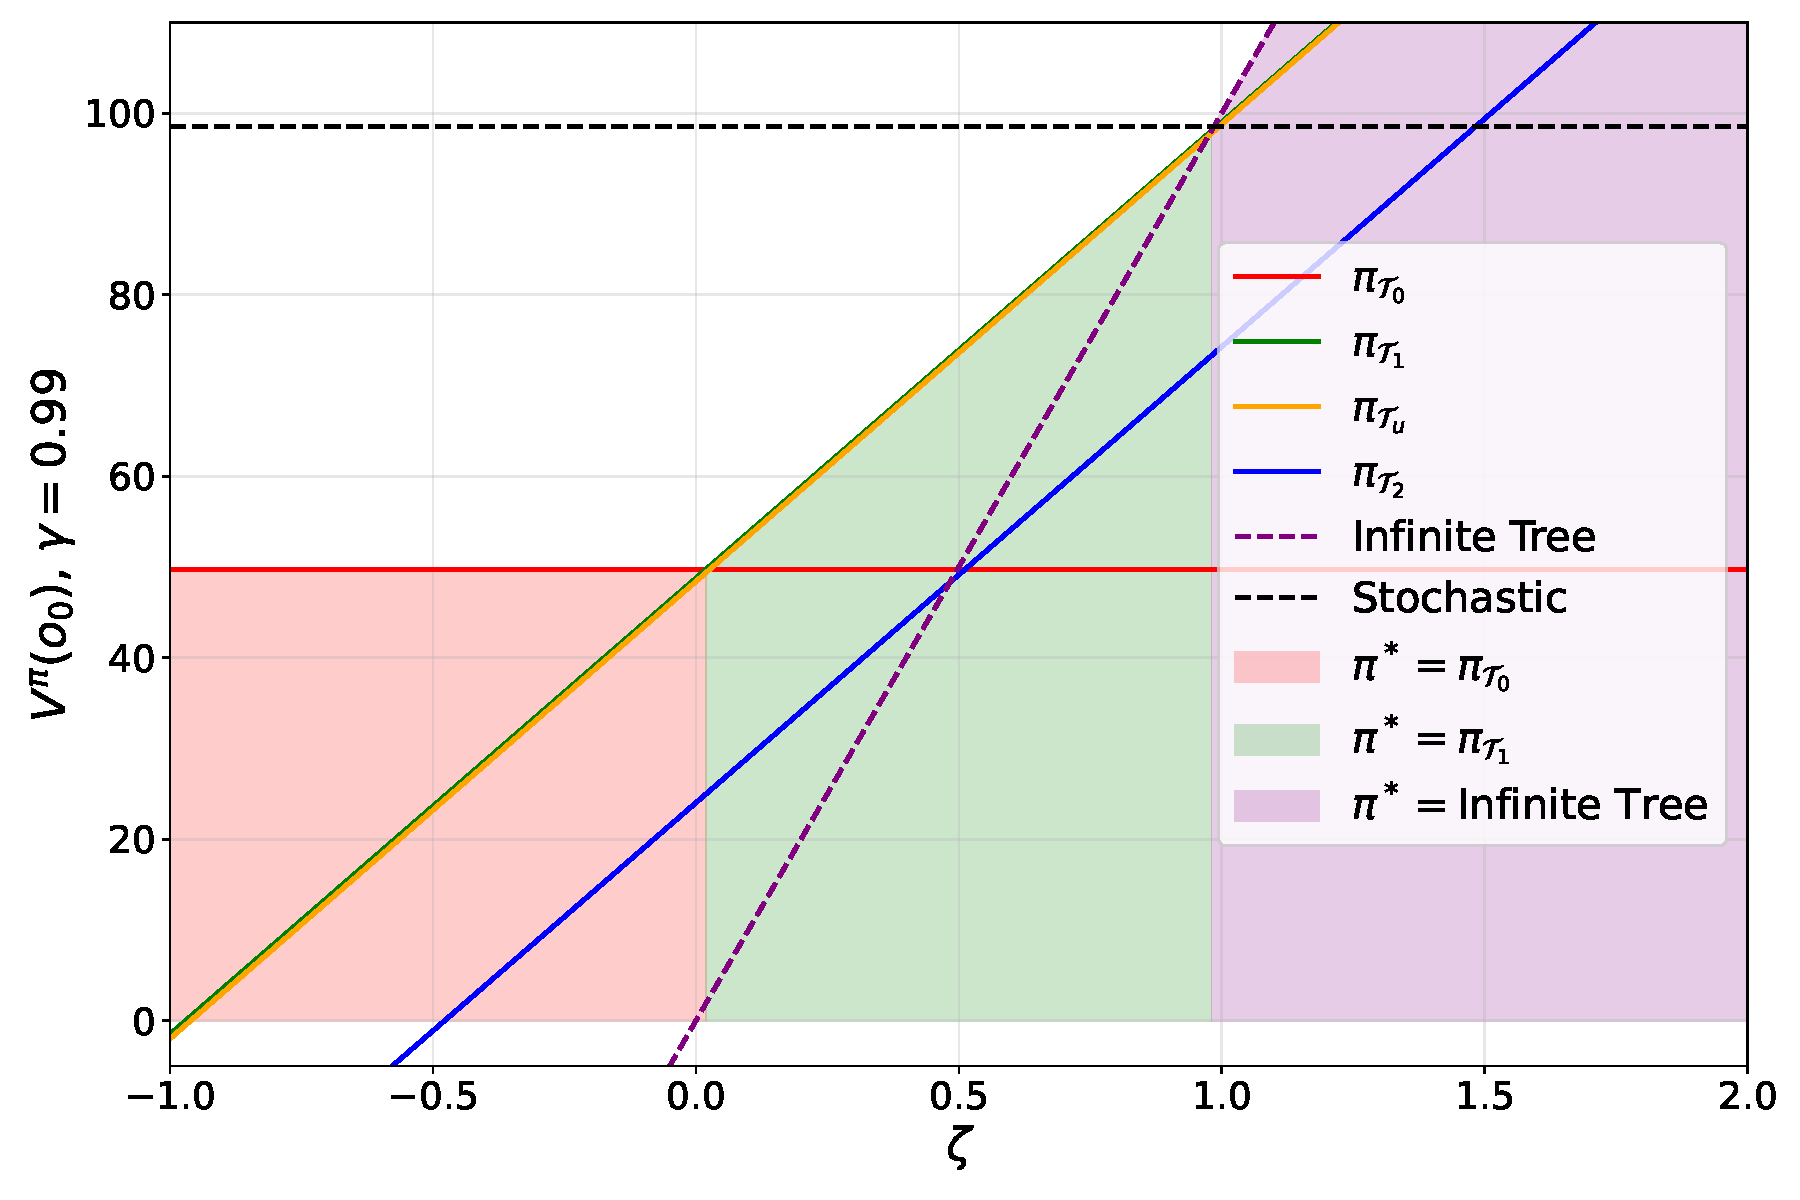
\includegraphics[width=1\textwidth]{images/images_part1/objective_values_plot.pdf}
    \caption{POIBMDP objective values of different policies as functions of $\zeta$. Shaded areas show the optimal policies in different ranges of $\zeta$ values.}\label{fig:objectives}
\end{figure}

We can now plot, in Figure (cite), the POIBMDP objective values of the different policies corresponding to trees for the grid world MDP as functions of $\zeta$ when we fix $\gamma=0.99$. 
When $\gamma=0.99$ on FIgure (cite), despite objective values being very similar for the depth-1 and unbalanced depth-2 tree, we now know from the green shaded area {\color{blue}a depth-1 tree is the optimal deterministic partially observable POIBMDP policy for $0< \zeta < 1$}.

Interestingly, two POMDP challenges described in (cite) can also be observed in Figure (cite). 
First, there is a whole range of $\zeta$ values for which the stochastic policy is optimal.
Second, for e.g. $\zeta=0.5$, while the depth-1 tree is the optimal deterministic partially observable policy, the value of state $(s_2, o_0) = (1.5, 1.5, 0, 2, 0, 2)$ is not maximized by this policy but by the sub-optimal policy that always goes down.

We can define a POIBMDP with the grid wolrd (cite) as base MDP, with IGAs as in the IBMDP from (cite), with $\gamma=0.99$ and $0<\zeta<1$ and verify if we can learn the optimal depth-1 decision tree.

\subsection{(Asymmetric) Reinforcement Learning in PO(IB)MDPs}

In general, the policy that maximizes the expected discounted cumulative reward in a POMDP maps ``belief states'' or observations histories (cite) to actions, i.e., they are not solutions to our problem (cite) since we require that policies depend only on the current observation.
If we did not have this constraint, we could apply any standard RL algorithm to solve POIBMDPs by seeking such policies because both histories and belief states are sufficient statistic for POMDPs hidden states (cite).

The particular, the problem of finding the optimal deterministic partially observable policies for POMDPs is NP-HARD, even with full knowledge of transitions and rewards (cite 3.2 littman). 

It means that, there is no reason to believe that any algorithm for solving it must enumerate all possible policies and take the best one. 
For even moderate-sized POMDPs, a brute-force approach will take a very long time since there are $|A|^{|O|}$ policies.

Hence it is interesting to study reinforcement learning for finding the best deterministic partially observable policy since it would not search the whole solution space.
However applying RL to problem (cite) is non-trivial.

In (cite), authors show that the optimal partially observable policy can be stochastic (cite precise section), hence policy gradient algoriothms (cite) are to prohibit since we want a \textit{deterministic} policy. 
Furthermore, the optimal deterministic patially observable policy might not maximize all the values of all observations simulataneously (cite precise section) which makes difficult to use TD-learning to learn policies.
Indeed, doing a TD-learning update of one partially observable value (cite) with, e.g. Q-learning (cite), can change the value of \textit{all} other observations in a unctrollable manner because of the depedence in $P^{\pi}((s, \boldsymbol{o}')|\boldsymbol{o})$ in (cite).

Despite those hardness results, empirical results of applying RL to POMDPs by naively replacing $\boldsymbol{x}$ by $\boldsymbol{o}$ in Q-learning (cite) or Sarsa (cite), has shown promising results (cite). 
More recently, the framework of Baisero et. al. (cite) called asymmetric RL has also shown promising results to learn POMDP solutions (cite)(see slides gaspard lambrechts nature).
Asymmetric RL trains a fully observable state-dependent model and a history-dependent (or observation-dependent) model informed by the former.
The history-dependent (or observation-dependent) model can thus be deplyed in the POMDP after training since it does not require access to the hidden fully observable state to output actions.
In Algorithms (cite) and (cite) we present asymmetric Q-learning and asymmetric Sarsa. Given a POMDP, e.g. a POIBMDP, both train an observation-dependet Q-function $Q:O\times A\rightarrow\mathbb{R}$ and a state-dependent Q-function $U:X\times A\rightarrow\mathbb{R}$.

In (cite), authors introduce policy search algorithm (cite) that learns a (stochastic) policy $\pi:O\rightarrow\Delta A$ and a critic (cite) $V:X\rightarrow \mathbb{R}$ using Monte Carlo estimates to guide policy improvement.
We write this algorithm that call JSJ (for the authors name Jakkola, Sing, Jordan) in Algorithm (cite). JSJ is equivalent to a tabular asymmetric policy gradient (cite) algorithm. 
\RestyleAlgo{ruled}
\SetKwComment{Comment}{}{}
\begin{algorithm}
    \KwData{POMDP $\mathcal{M}_{po} = \langle X, O, A, R, T, T_0, \Omega \rangle$, learning rates $\alpha_u,\quad \alpha_q$, exploration rate $\epsilon$}
    \KwResult{$\pi:O\rightarrow A$}
    Initialize $U(x,a) = 0$ for all $x \in X, a \in A$ \\
    Initialize $Q(o,a) = 0$ for all $o \in O, a \in A$ \\

    \For{each episode}{
        Initialize state $x_0 \sim T_0$ \\
        Initialize observation $o_0 \sim \Omega(x_0)$ \\

        \For{each step $t$}{
            Choose action $a_t$ using $\epsilon$-greedy: $a_t = \arg\max_a Q(o_t,a)$ with prob. $1-\epsilon$ \\
            Take action $a_t$, observe $r_t = R(x_t,a_t)$, $x_{t+1} \sim T(x_t,a_t)$, and $o_{t+1} \sim \Omega(x_{t+1})$ \\
            $y \leftarrow r + \gamma U(x_{t+1}, \argmax_{a'} Q(o_{t+1}, a'))$ \Comment{// TD target} \\
            $U(x_t,a_t) \leftarrow (1 - \alpha_u) U(x_t, a_t) + \alpha_u y $ \\
            $Q(o_t,a_t) \leftarrow (1 - \alpha_q) Q(o_t, a_t) + \alpha_q y $ \\
            $x_t \leftarrow x_{t+1}$ \\
            $o_t \leftarrow o_{t+1}$ \\
        }
    }
    $\pi(o) = \arg\max_a Q(o,a)$ \Comment{// Extract greedy policy}
    \caption{Asymmetric Q-Learning (cite)}\label{alg:asymqlearning}
\end{algorithm}


\RestyleAlgo{ruled}
\SetKwComment{Comment}{}{}
\begin{algorithm}
    \KwData{POMDP $\mathcal{M}_{po} = \langle X, O, A, R, T, T_0, \Omega \rangle$, learning rates $\alpha_u,\quad \alpha_q$, exploration rate $\epsilon$}
    \KwResult{$\pi:O\rightarrow A$}
    Initialize $U(x,a) = 0$ for all $x \in X, a \in A$ \\
    Initialize $Q(o,a) = 0$ for all $o \in O, a \in A$ \\

    \For{each episode}{
        Initialize state $x_0 \sim T_0$ \\
        Initialize observation $o_0 \sim \Omega(x_0)$ \\

        \For{each step $t$}{
            Choose action $a_t$ using $\epsilon$-greedy: $a_t = \arg\max_a Q(o_t,a)$ with prob. $1-\epsilon$ \\
            Take action $a_t$, observe $r_t = R(x_t,a_t)$, $x_{t+1} \sim T(x_t,a_t)$, and $o_{t+1} \sim \Omega(x_{t+1})$ \\
            $y \leftarrow r + \gamma U(x_{t+1}, \argmax_{a'} Q(o_{t+1}, a'))$ \Comment{// TD target} \\
            $U(x_t,a_t) \leftarrow (1 - \alpha_u) U(x_t, a_t) + \alpha_u y $ \\
            $Q(o_t,a_t) \leftarrow (1 - \alpha_q) Q(o_t, a_t) + \alpha_q y $ \\
            $x_t \leftarrow x_{t+1}$ \\
            $o_t \leftarrow o_{t+1}$ \\
        }
    }
    $\pi(o) = \arg\max_a Q(o,a)$ \Comment{// Extract greedy policy}
    \caption{Asymmetric Sarsa (cite)}\label{alg:asymsarsa}
\end{algorithm}

\RestyleAlgo{ruled}
\SetKwComment{Comment}{}{}
\begin{algorithm}
    \KwData{POMDP $\mathcal{M}_{po} = \langle X, O, A, R, T, T_0, \Omega \rangle$, learning rate $\alpha$, policy parameters $\theta$, number of trajectories $N$}
    \KwResult{Stochastic partially observable policy $\pi_\theta: O\rightarrow \Delta A$}
    Initialize policy parameters $\theta$ \\
    Initialize $Q(o, a) = 0$ for all observations $o$ and actions $a$ \\
    \For{each episode}{
        \For{$i = 1$ to $N$}{
            Generate trajectory $\tau_i = (s_0, a_0, r_0, s_1, a_1, r_1, \ldots, s_T)$ following $\pi_\theta$ \\
            \For{each timestep $t$ in trajectory $\tau_i$}{
                $G_t \leftarrow \sum_{k=t}^{T} \gamma^{k-t} r_k$ \Comment{// Compute return}
                Store $(o_t, a_t, G_t)$ for later averaging
            }
        }
        \For{each unique observation-action pair $(o, a)$}{
            $Q(o, a) \leftarrow \frac{1}{|\{(o, a)\}|} \sum_{(o, a, G)} G$ \Comment{// Monte Carlo estimate}
        }
        \For{each observation $o$}{
            \For{each action $a$}{
                $\pi_1(a|o) \leftarrow 1.0$ if $a = \argmax_{a'} Q(o, a')$, $0.0$ otherwise \Comment{// Deterministic policy from Q-values}
                $\pi(a|o) \leftarrow (1 - \alpha) \pi(a|o) + \alpha \pi_1(a|o)$ \Comment{// Policy improvement step}
            }
        }
        Reset $Q(o, a) = 0$ for all observations $o$ and actions $a$ \Comment{// Reset for next episode}
    }
    \caption{JSJ algorithm. Uses Monte Carlo estimates of the average reawrd value functions to perform policy imporvements (cite)}\label{alg:jsj}
\end{algorithm}

Until recently the benefits of asymmetric RL over standard RL was only shown empirically and only for history-dependent models.
The work of Gaspard Lambrechts (cite thesis and article) proves that some asymmetric RL algorithms learn better history-dependent \textbf{or} observation-dependent policies for solving POMDPs.
This is exactly what we wish however those algorithms are intractable in practice because they require estimation of the quantity $P^{\pi}((s, \boldsymbol{o}')|\boldsymbol{o})$.
We leave it to future work to use those algorithms that combine asymmetric RL and estimation of future visitations since those result are contemporary to the writing of this manuscript.

We still try vanilla asymmetric Q-learning and vanilla asymmetric Policy Gradient (cite) and we already tried, in the previous chapter, modified DQN (cite) and modified PPO (cite) that are respectively Asymmetric DQN (cite) and Asymmetric (PPO) from (cite) and (cite).

\section{Results}

Unfortunately, our results are negative and show that (asymmetric) reinforcement learning fails for the aforementioned problem. Let us understand why.

\subsection{Experimental Setup}

\paragraph{Baselines:} we consider two groups of RL algorithms. The first group is standard tabular RL naively applied to POIBMDPs; Q-learning (cite)(cite), Sarsa (cite)(cite), and Policy Gradient (cite)(cite).
(cite) and (cite) already studied the theoretical and practical implications of applying standard RL directly to POMDP by considering that partial observations are full MDP states.
(cite) proved that Q-Learning will converge but without optimality guarantees. 
(cite) showed empirically that Sarsa-$\lambda$ (cite), a version of Sarsa with some sort of memory, can learn good deterministic solutions to POMDP which makes it a good candiate for our problem.

We also use a vanilla tabular Policy Gradient baseline (cite) with softmax policy, which to the best of our knowledge, nobody studied in our setting.
In theory the Policy Gradient algorithm should not be a good candidate for our problem since it searches for stochastic policies that we showed can be better than our seeked depth-1 decision tree policy (c.f. Figure (cite)).

More recently, RL algorithms were developped specially for learning policies in POMDPs. Those algorithms are called asymmetric RL which authors of the original IBMDP paper (cite) use without knowing. 
Asymmetric algorithms leverage the fact that, even if the deployed policy should depend only on partial observation, nothing forbids the use of full state information during training if the latter is available.
Asymmetric Q-learning (cite) makes use of full-state-action value function $U:S\times O \timesA \rightarrow \mathbb{R}$ to use as a temporal difference error target (cite) when updating the $Q:O\times A\rightarrow \mathbb{R}$ of intereset. 
In Algorithm (cite), we write the Asymmetric Q-learning algorithm.    

In addition to the traditional tabular RL algorithms, we also apply Asymmetric Q-learning and Asymmetric Sarsa and JSJ, the tabular algorithm from (cite)(cite) which is equivalent to a tabular Asymmetric Policy Gradient algorithm.

We use at least 200 000 time steps to train each agent. Each agent is trained on 100 seeds on each POIBMDP.  

\paragraph{Hyperparameters:} For all baselines we use, when applicable, exploration rates $\epsilon=0.3$ and learning rates $\alpha=0.1$.

\paragraph{Metrics:} we will consider two metrics.
First, the sub-optimality gap of the learned policy POIBMDP value with respect to the optimal deterministic partially observable POIBMP policy: $|V^\pi^{\star}(o_0) - V^\pi(o_0)|$
Because we know the whole POIBMDP model that we can represent exactly as tables; and because we know for each $\zeta$ value the POIBMDP objective value of the optimal partially observable policy (c.f. Figure); we can report the \textit{exact} sub-optimality gaps.

Second, we consider the distribution of the learned trees structure over the 100 training seeds.
Indeed, since for every POIBMDP we train each baseline 100 times, we obtain 100 partially observable deterministic policies from which we can extract the equivalent 100 decision tree policies using Algorithm (cite).
This helps understand which trees RL tend to learn.

\subsection{Can RL baselines find the optimal deterministic partially observable POIBMDP policies?}

In Figure (cite), we plot the sub-optimality gaps--averaged over 100 seeds--of learned policies during training.
We do so for 200 different POIBMDPs where we change the reward for information gathering actions: we sample $\zeta$ uniformily in $[-1, 2]$.
For (asymmetric) Q-learning and (asymmetric) Sarsa, we extract the greedy policies from the learned Q-functions and evaluate them every 2000 steps.
For the Policy Gradient and the JSJ baselines we directly evaluate the learned stochastic policies.

In Figure (cite), we plot the distributions over the final learned trees in function of $\zeta$ from the above runs.
For the Policy Gradient and JSJ baselines, we extract the tree from the policy that is greedy w.r.t to the action probabilities as ALgorithm 6 requires a deterministic partially observable policy to return a tree policy.

We observe that, despite all runs converging, independently of the $\zeta$ values, not all runs fully minimize the sub-optimality gap.
In particular all RL algorithms seem to consistantly minimze the gap, i.e. learn the optimal policy or Q-function, for $\zeta \in [-1, 0]$, where the optimal policy is the detph-0 tree.
For $\zeta \in [1, 2]$, where the optimal policy is to repeat taking information gathering actions, only the Q-learning baseline learns the optimal policy. 
In $\zeta \in ]0, 1[$, where the depth-1 tree is optimal, no baseline can consistently learn the optimal solution. However, we observe that asymmetric versions of Q-learning and Sarsa have found the optimal policy more frequently than other baselines.
One interpretation of this phenomenon is that the learning in POIBMDPs is very difficult and so agents tend to converge to trivial policies, e.g., repeating the same base action.

Next, we quantify how difficult it is to do RL to learn policies in POIBMDPs.
\begin{figure}
    \centering
    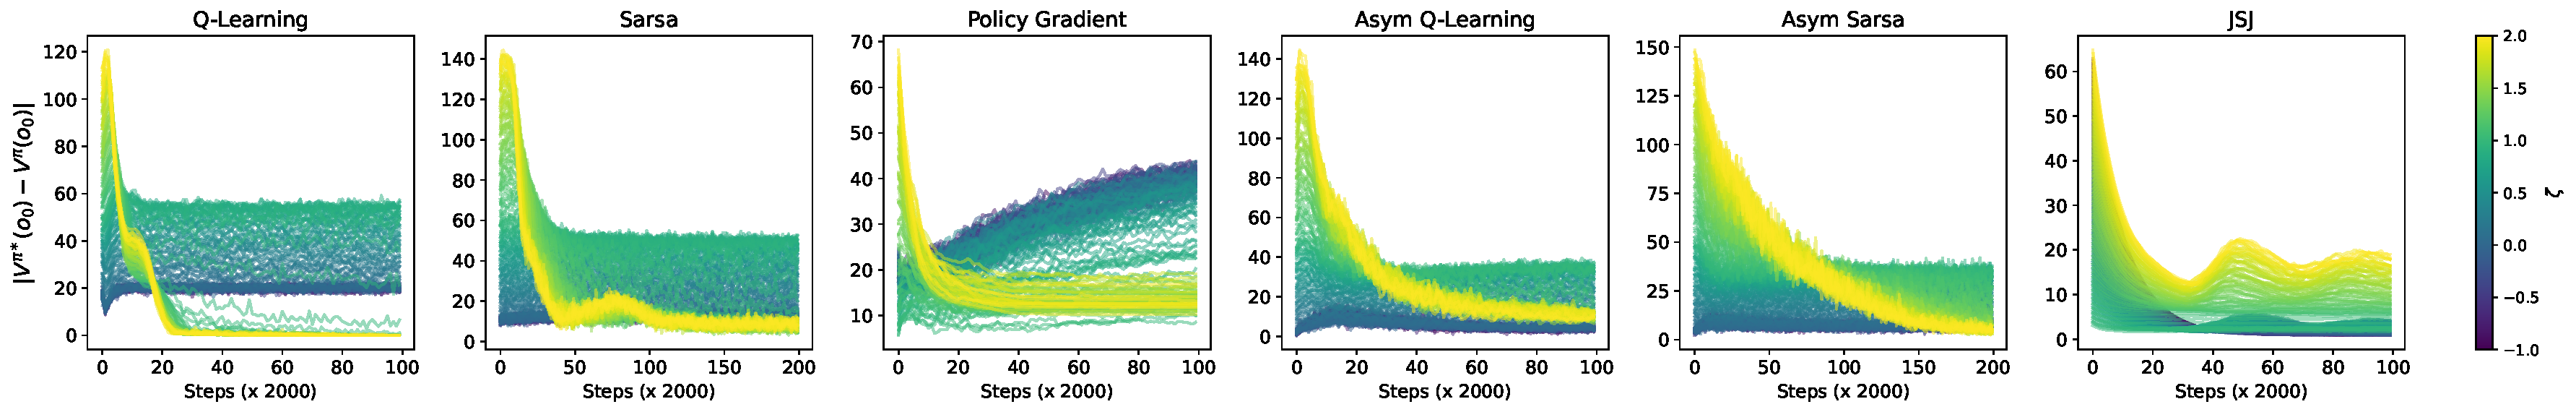
\includegraphics[width=1\textwidth]{images/images_part1/learning_curves.pdf}
    \caption{Baselines learning curves of partially observable policies in POIBMDPs. 
    In each subplot, each single learning curve is colored by the value of $\zeta$ in the corresponding POIBMDP in which learning occurs. 
    Each single learning curve represent the sub-optimality gap averaged over 100 seeds.
    So for each baseline we ran a total of $200 \times 100$ single training run.
    }\label{fig:rl-poibmdp}
\end{figure}

\begin{figure}
    \centering
    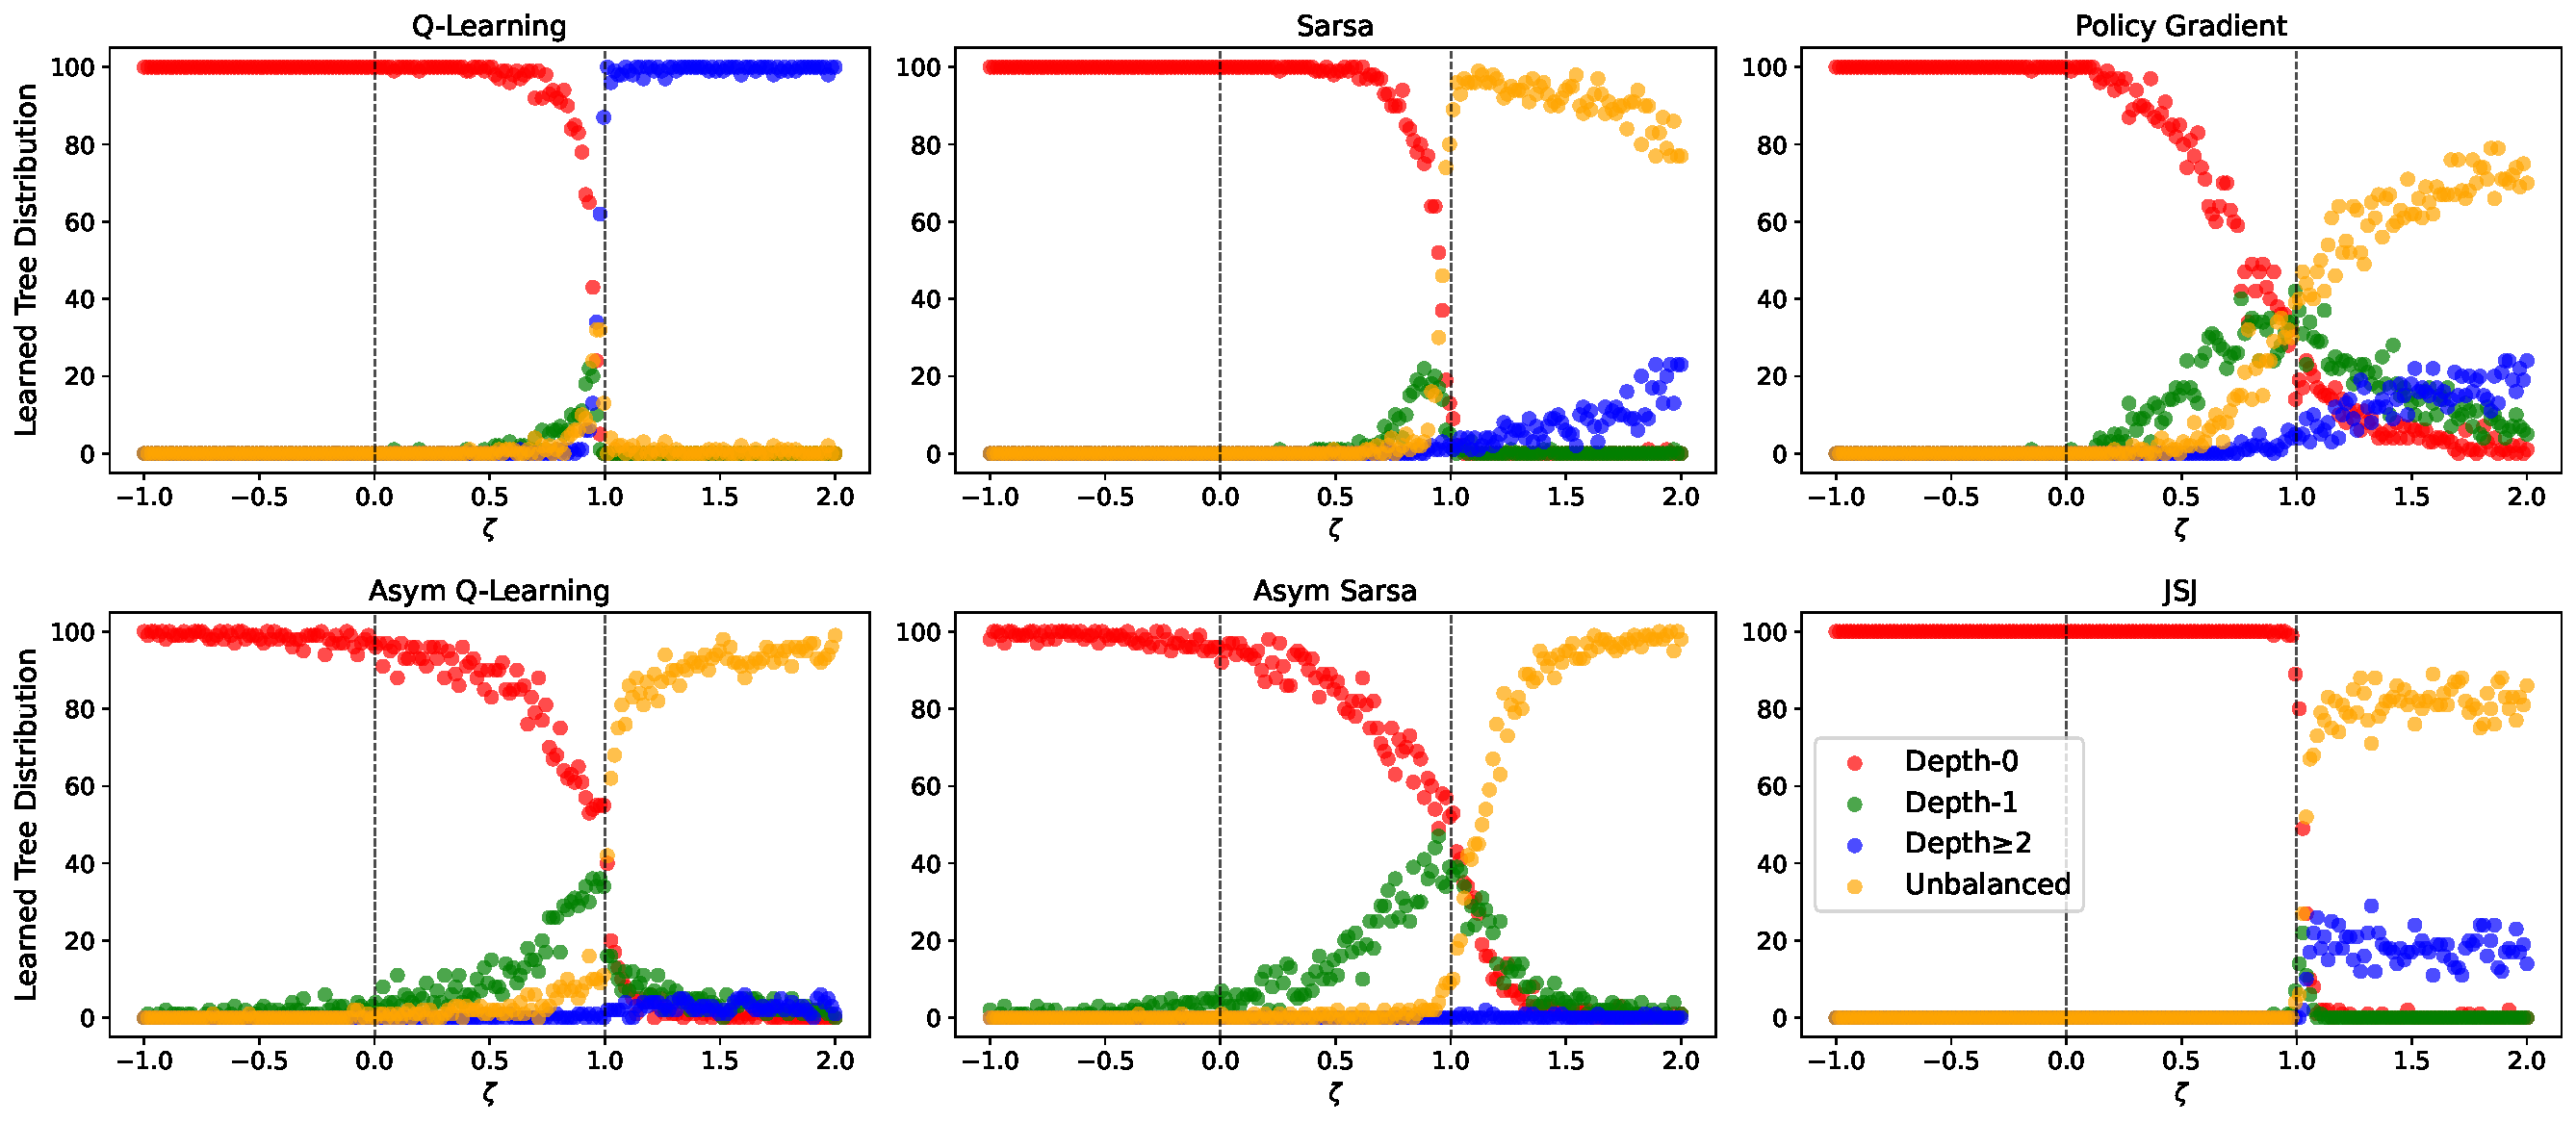
\includegraphics[width=1\textwidth]{images/images_part1/tree_distributions.pdf}
    \caption{Distributions of final tree policies learned across the 100 seeds.
    For each $\zeta$ value, there are four color points each represeting the share of depth-0 trees (red), depth-1 trees (green), unbalanced depth-2 trees (orange) and depth-2 trees (blue).
    Note that those tres do not necessary correspond to tres in Figure (cite). We simply check the structure of trees and not if they are the best-in-class tree. 
    }\label{fig:dt-distrib-poibmdp}
\end{figure}


\subsection{How difficult is it to learn in POIBMPDs?}

To show that learning the optimal deterministic partially observable POIBMDP policy is very difficult, even though there are only a handful of states, observations, and actions (16, 9, and 6 respectively), we compare the success rate of RL baselines when applied to a POIBMDP with $\gamma=0.99$, $\zeta=0.5$ and when applied to the corresponding fully observable IBMDP, and MDP.

Because we know that for those values of $\zeta$ and $\gamma$, the optimal deterministic partially observable policy is a depth-1 tree and the optimal fully observable policy is a tabular policy from Figure (cite); we can compute the success rate of an algorithm as the proportion of learned policies that match their optimal counterparts.

Furhtermore; we also consider advanced tricks for tabular RL in order to properly assess the difficulty of learning in POIBMDPs compared to learning in (IB)MDPs:
\begin{enumerate}
    \item Optimistic Q-function (cite)
    \item Entropy regularization (cite)
    \item Eligibility traces (cite)
    \item $\epsilon$-decay (cite)
\end{enumerate}
In particular, for each of the aforementioned RL baselines; we learn policies using a wide variety of hyperparamters.
For example, in Table (cite) we provide the detailed hyperparameter space of Asymmetric Sarsa, which induce a total of 1152 instances of Asymmetric Sarsa, and in Table (cite) we provide the hyperparameter space sizes for all baselines.
We run each baseline using each hyperparamters combination 10 times on 200000 timesteps.

\begin{table}[h]
\centering
\caption{Asymmetric Sarsa Hyperparameter Space (768 combinations each run 10 times)}
\begin{tabular}{lll}
\toprule
\textbf{Hyperparameter} & \textbf{Values} & \textbf{Description} \\
\midrule
Epsilon Schedules & (0.3, 1), (0.3, 0.99), (1, 1) & Initial exploration and decrease rate \\
Epsilon Schedules & (0.1, 1), (0.1, 0.99), (0.3, 0.99) & Initial exploration and decrease rate \\
Lambda & 0.0, 0.3, 0.6, 0.9 & Eligibility trace decay \\
Learning Rate $U$ & 0.001, 0.005, 0.01, 0.1 & $Q$ learning rate \\
Learning Rate $Q$ & 0.001, 0.005, 0.01, 0.1 & $U$ learning rate \\
Optimistic & True, False & Optimistic initialization \\
\bottomrule
\end{tabular}
\end{table}

\begin{table}[h]
    \centering
    \caption{Summary of RL baselines Hyperparameters}
    \begin{tabular}{llr}
    \toprule
    \textbf{Algorithm} & \textbf{Problem} & \textbf{Total Hyperparameter Combinations} \\
    \midrule
    Policy Gradient & PO/IBMDP & 420 \\
    JSJ & POIBMDP & 15 \\
    Q-learning & PO/IBMDP & 192 \\
    Asym Q-learning & POIBMDP & 768 \\
    Sarsa & PO/IBMDP & 192 \\
    Asym Sarsa & POIBMDP & 768 \\
    \bottomrule
    \end{tabular}
    \end{table}


\begin{figure}
    \centering
    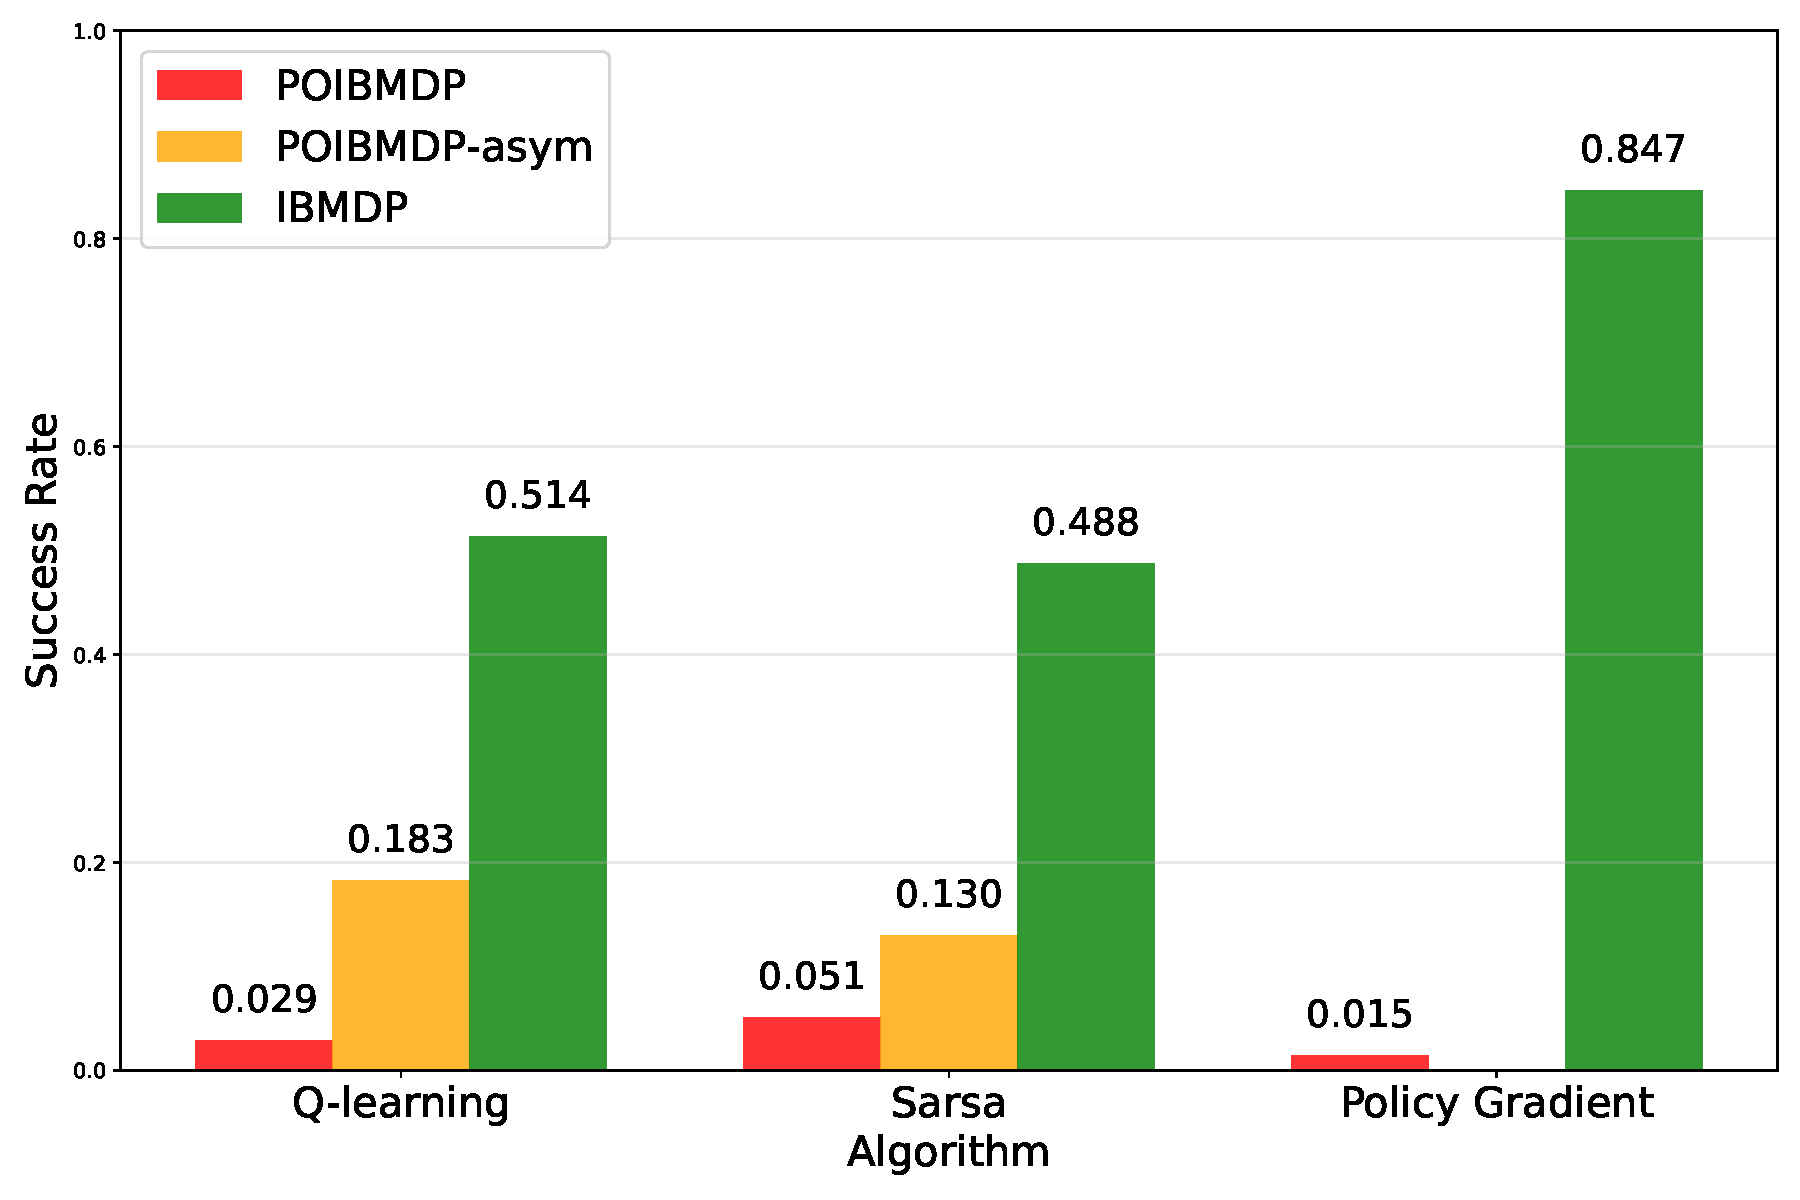
\includegraphics[width=1\textwidth]{images/images_part1/algorithm_performance_comparison_flattened.pdf}
    \caption{Success rates of different RL algorithms over thousands of runs when applied to a POIBMDP and its fully observable IBMDP and MDP counterparts}\label{fig:po-vs-ib}
\end{figure}


\begin{table}[h]
    \centering
    \begin{tabular}{|l|c|c|c|}
    \textbf{Hyperparameter} & \textbf{Asym Q-learning (10/10)} & \textbf{Asym Sarsa (10/10)} & \textbf{PG (4/10)} \\
    \toprule
    epsilon\_start & 1.0 & 1.0 & - \\
    epsilon\_decay & 0.99 & 0.99 & - \\
    batch\_size & 1 & 1 & - \\
    lambda\_ & 0.0 & 0.0 & - \\
    lr\_o & 0.01 & 0.1 & - \\
    lr\_v & 0.1 & 0.005 & - \\
    optimistic & False & False & - \\
    lr & - & - & 0.05 \\
    tau & - & - & 0.1 \\
    eps & - & - & 0.1 \\
    n\_steps & - & - & 2000 \\
    \bottomrule
    \end{tabular}
    \caption{Best hyperparameters for each algorithm on the POIBMDP problem}
    \label{tab:algorithm-hyperparameters}
    \end{table}

\begin{figure}
    \centering
    \begin{subfigure}[b]{0.32\textwidth}
        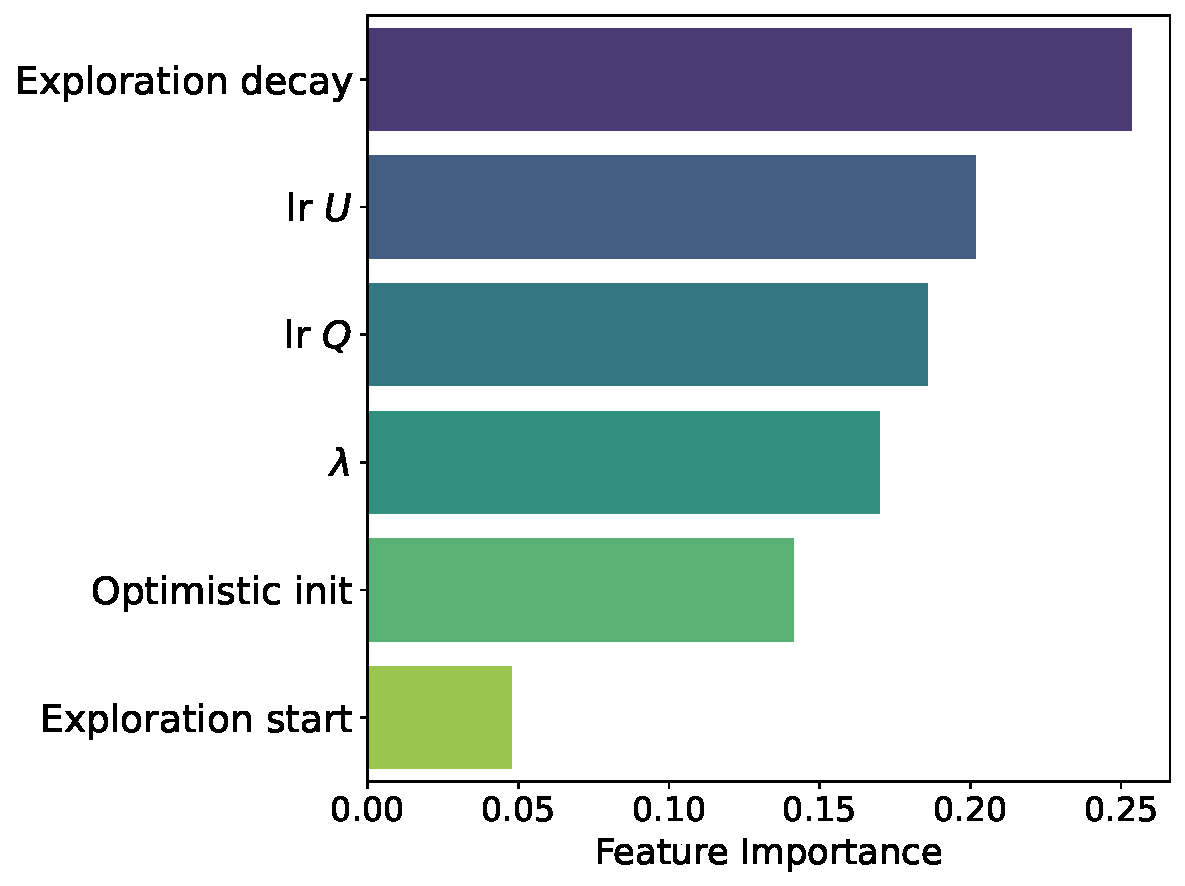
\includegraphics[width=\textwidth]{images/images_part1/hyperparameter_importance_ql_asym.pdf}
        \caption{Hyperparameter importance for Asymmetric Q-learning}
        \label{fig:hyperparam-importance}
    \end{subfigure}
    \hfill
    \begin{subfigure}[b]{0.32\textwidth}
        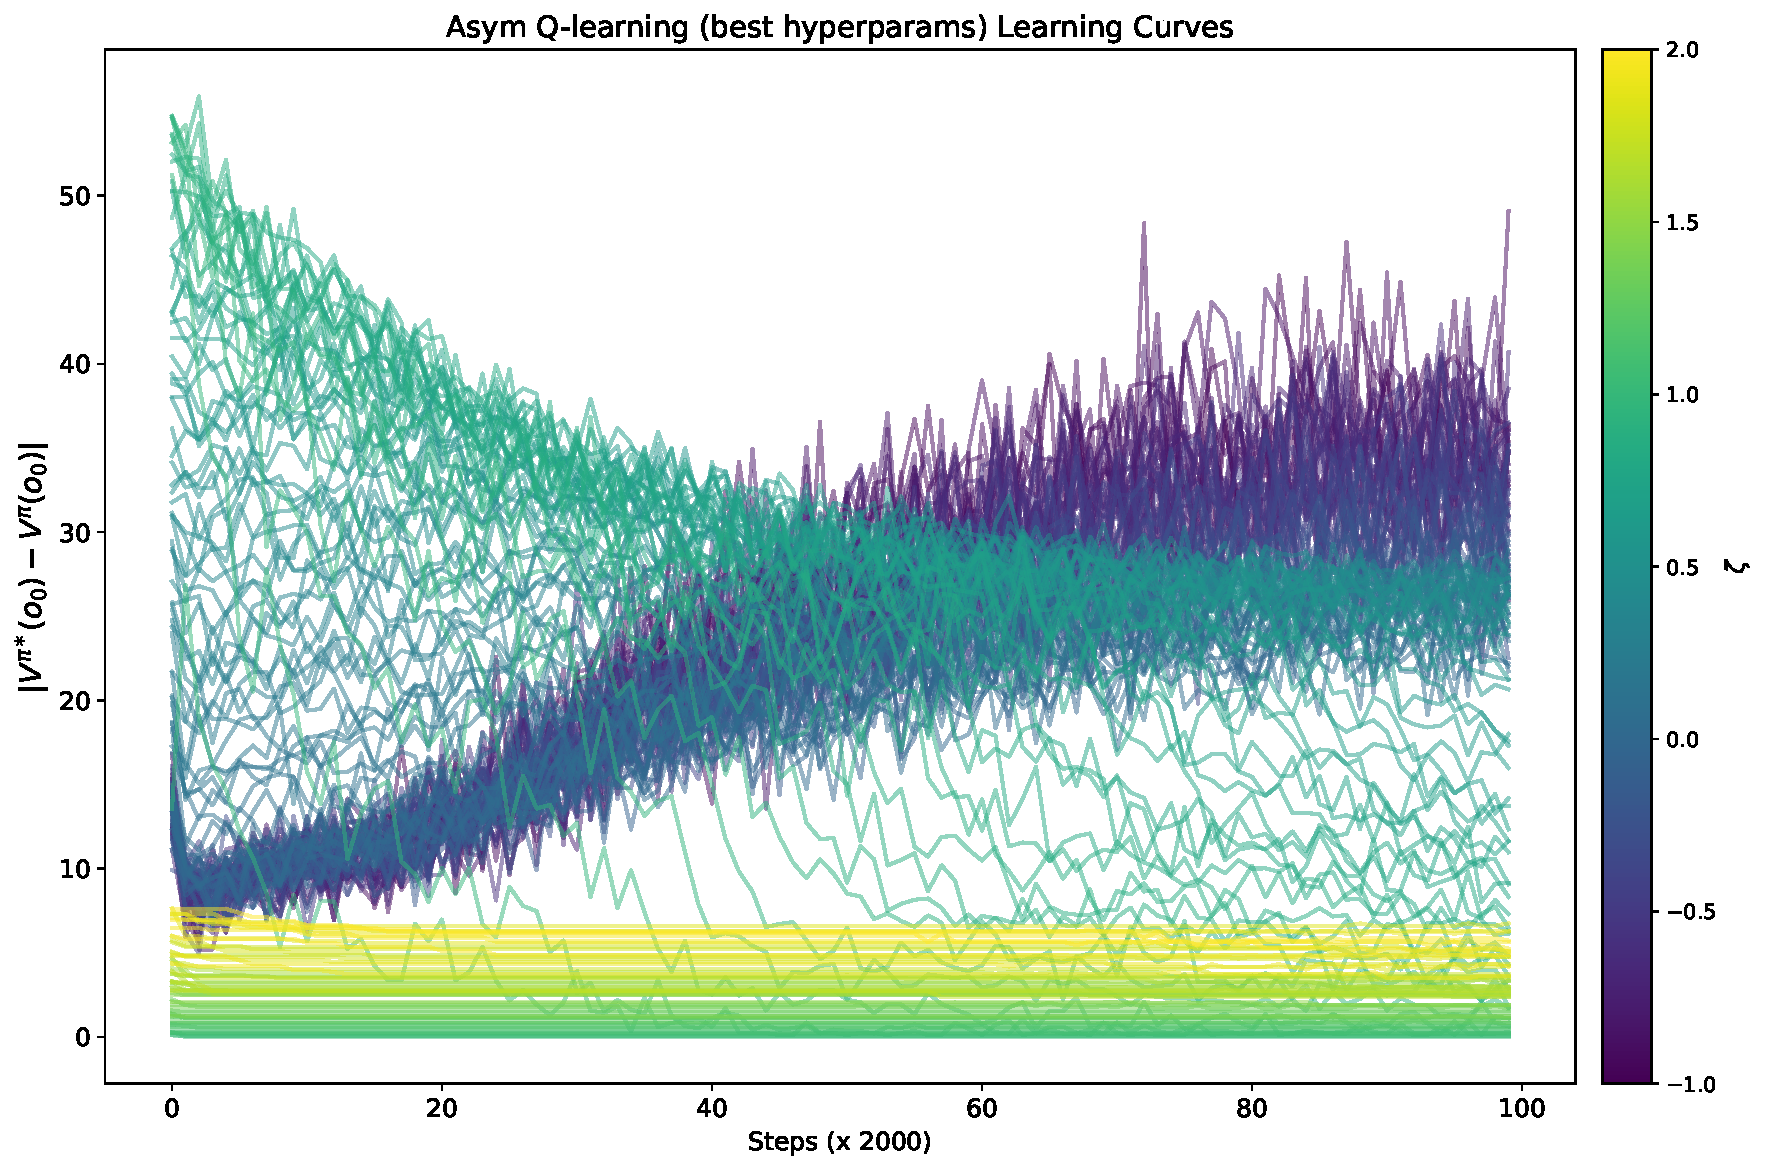
\includegraphics[width=\textwidth]{images/images_part1/ql_asym_best_learning_curves.pdf}
        \caption{Best learning curves for Asymmetric Q-learning}
        \label{fig:best-learning-curves}
    \end{subfigure}
    \hfill
    \begin{subfigure}[b]{0.32\textwidth}
        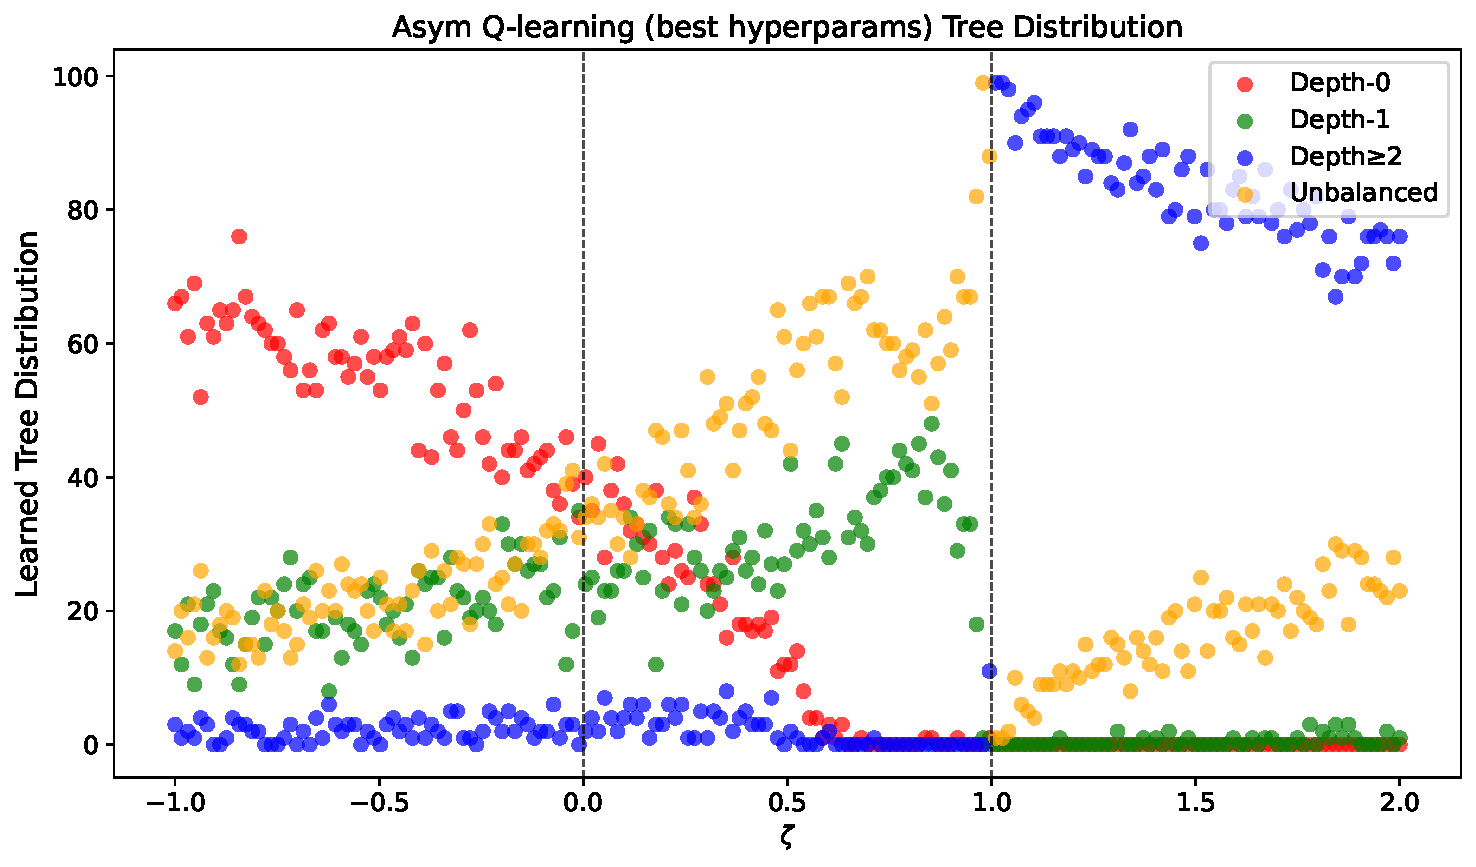
\includegraphics[width=\textwidth]{images/images_part1/ql_asym_best_tree_distributions.pdf}
        \caption{Best tree distributions for Asymmetric Q-learning}
        \label{fig:best-tree-distributions}
    \end{subfigure}
    \caption{Asymmetric Q-learning performance analysis: hyperparameter importance, learning curves, and tree distributions across different POIBMDP configurations.}
    \label{fig:asym-ql-analysis}
\end{figure}


The key observations from Figure (cite) is that POIBMDPs are way harder than their IBMDPs counterparts.
Even though asymmetry seems to increase performances; learning a decision tree policy for a simple grid world directly with RL using the framework of POIBMDP seem way to difficult and costly as successes might require a million steps for such a seemingly simple problem.
An other difficulty in practice that we did not cover is the choice of information gathering actions.
For the grid world MDP, choosing good IGAs ($x\leq1$ and $y\leq1$) is simple but what about more complicated MDPs? 
Even after choosing candidate IGAs; RL with large action space is known to be an already difficult problem.

It is important to note that some hyperparameter sets gave a 10/10 success rate for asymmetric baselines (c.f. Table (cite)). 
However, when we try those top performing hyperparameters on more seeds, as shown in Figure (cite), even though we observe an increase in the proportion of depth-1 trees learned, the performance are still not satisfactory for such a simple task. 

\section{Conclusion}
In this Chapter, we have shown that direct learning of decision tree policies for MDPs can be reduced to learning deterministic partially observable policies in POMDPs. 
We once again showed the difficulty of the latter by crafting a POIBMDP for which we know exactly the optimal deterministic partially observable policy.
This allowed to show 1) that existing (asymmetric) RL algorithms fail to consistently learn the optimal deterministic partially observable policy (c.f. Figure (cite)) and 2) to show that for similar transitions and rewards, learning a partially observable deterministic policy is way harder than learning a fully observable one (c.f. Figure (cite)).

So interesting future work could be to design POIBMDP-specific algorithm or to find another framework for the direct learning of decision trees for MDPs.
Overall, in the two last Chapter, it seems fair to say that indirect interpretability is more suited for MDPs
Despite those negative conclusion, there is still some positive directions coming out of this work.
In the next Chapter, we show that when the base MDP's transitions are independent of the action, then POIBMDPs are actually \textit{fully} observable which can lead to new decision tree induction for supervised learning.